\documentclass[12pt]{article}
\usepackage{amsmath}
\usepackage{amssymb}
\usepackage[letterpaper,margin=0.85in,centering]{geometry}
\usepackage{fancyhdr}
\usepackage{enumerate}
\usepackage{lastpage}
\usepackage{multicol}
\usepackage{graphicx}

\reversemarginpar

\pagestyle{fancy}
\cfoot{}
\lhead{Math 1560}\chead{Tutorial Assignment \# 8 Solutions}\rhead{June 6th, 2017}
%\rfoot{Total: 10 points}
%\chead{{\bf Name:}}
\newcommand{\points}[1]{\marginpar{\hspace{24pt}[#1]}}
\newcommand{\skipline}{\vspace{12pt}}
%\renewcommand{\headrulewidth}{0in}
\headheight 30pt

\newcommand{\di}{\displaystyle}
\newcommand{\abs}[1]{\left\lvert #1\right\rvert}
\newcommand{\len}[1]{\lVert #1\rVert}
\renewcommand{\i}{\mathbf{i}}
\renewcommand{\j}{\mathbf{j}}
\renewcommand{\k}{\mathbf{k}}
\newcommand{\R}{\mathbb{R}}
\newcommand{\aaa}{\mathbf{a}}
\newcommand{\bbb}{\mathbf{b}}
\newcommand{\ccc}{\mathbf{c}}
\newcommand{\dotp}{\boldsymbol{\cdot}}
\newcommand{\bbm}{\begin{bmatrix}}
\newcommand{\ebm}{\end{bmatrix}}                   
                  
\begin{document}

%\author{Instructor: Sean Fitzpatrick}
\thispagestyle{fancy}
%\noindent{{\bf Name and student number:}}

\begin{enumerate}
 \item A woman throws a stick into a lake for her dog to fetch; the stick is 15 feet down the shore line and 30 feet into the water from there. The dog may jump directly into the water and swim, or run along the shoreline to get closer to the stick before swimming. The dog runs about 22 ft/s and swims about 1.5 ft/s.

How far along the shore should the dog run to minimize the time it takes to get to the stick?

\medskip

\begin{multicols}{2}
 \begin{center}
  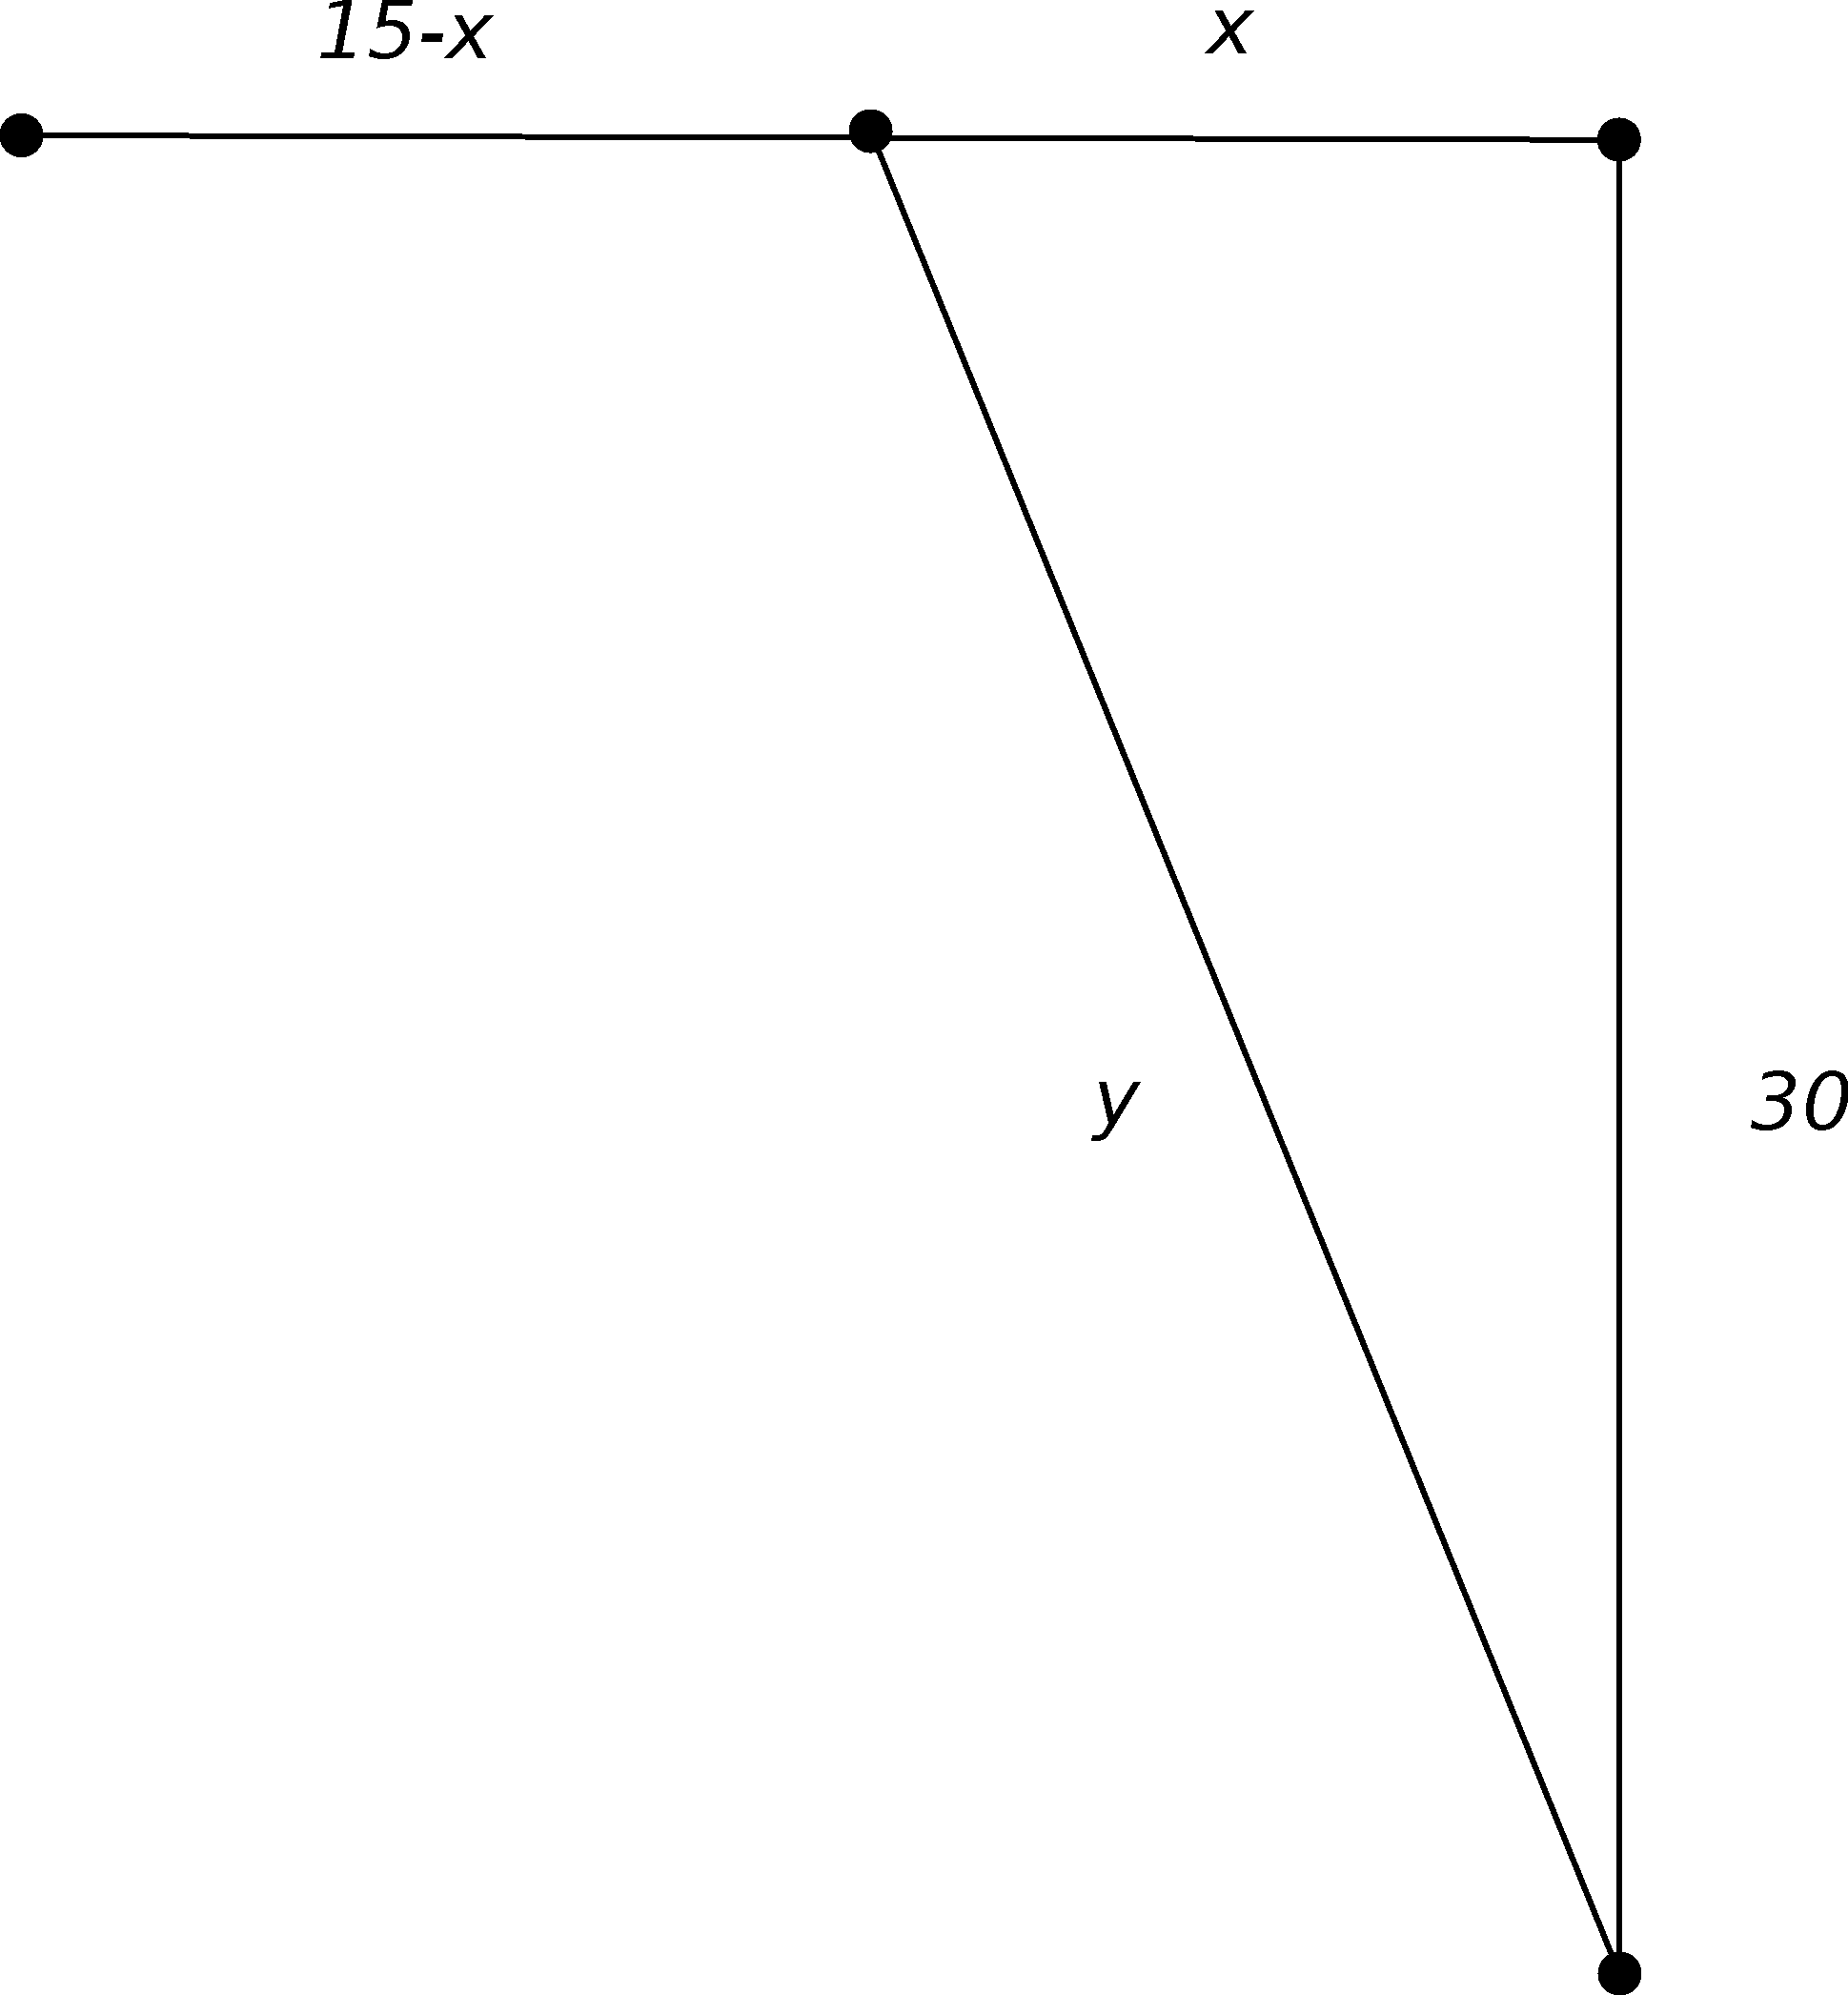
\includegraphics[width=0.6\columnwidth]{WS8-1sol}
 \end{center}
 \columnbreak
 Referring to the diagram to the left, we let $x$ be the distance remaining in the total of 15 feet when the dog enters the water, so that the dog runs a distance of $15-x$, and swims a distance of $y=\sqrt{x^2+30^2}$. Since time is given by distance divided by speed, the total time it takes the dog to reach the stick is
\[
 t = \frac{15-x}{22}+\frac{\sqrt{x^2+30^2}}{1.5} = \frac{15-x}{22}+\frac{2(x^2+30^2)^{1/2}}{3}.
\]
\end{multicols}
The derivative of $t$ with respect to $x$ is then
\[
 \frac{dt}{dx} = -\frac{1}{22}+\frac{2}{3}\cdot\frac{1}{2}(x^2+30^2)^{-1/2}(2x) = \frac{44x-3\sqrt{x^2+30^2}}{66\sqrt{x^2+30^2}}.
\]
We thus have $\frac{dt}{dx}=0$ when $44x-3\sqrt{x^2+30^2}=0$, or $44x=3\sqrt{x^2+30^2}$. Squaring both sides of this equation (which is valid, since $x\geq 0$), we get
\[
 44^2x^2=9(x^2+30^2) \quad \Rightarrow \quad (44^2-9)x^2 = 9(30^2) = (90)^2.
\]
Solving for $x$ (and taking the positive root, since $x\geq 0$), we have
\[
 x = \frac{90}{\sqrt{44^2-9}}\approx 2.05.
\]
The distance the dog should run is therefore $15-2.05 = 12.95$ feet.

\bigskip

 \item Use a linear approximation (differential) to estimate the value of $\sqrt[3]{8.06}$.

\medskip

 We note that $\sqrt[3]{8.06} = f(8.06) = f(8+0.06)$ for the function $f(x)=\sqrt[3]{x} = x^{1/3}$. Since we know that $f(8) = \sqrt[3]{8}=2$, we use a linear approximation near $a=2$. We find $f'(x) = \frac{1}{3}x^{-2/3}$, so
\[
 f'(8) = \frac{1}{3(8^{2/3})} = \frac{1}{3\cdot 4} = \frac{1}{12}.
\]
Our approximating function is therefore $l(x) = 2+\frac{1}{12}(x-8)$, giving us the approximation
\[
 f(8.06) \approx l(8.06) = 2+\frac{1}{12}(8.06-8) = 2+\frac{1}{12}\left(\frac{6}{100}\right) = 2+\frac{1}{200} = 2+0.005 = 2.005.
\]
(A more precise approximation, from the calculator, is $\sqrt[3]{8.06}\approx 2.004987552$.)

\newpage

 \item Let $f(x) = \ln(x+1)$.
\begin{enumerate}
 \item Calculate the degree 4 Taylor polynomial of $f$ about $a=0$.

\medskip

We begin by computing our coefficients:
\[
\begin{array}{lll}
 f(x) = \ln(x+1) & f(0) = 0 & a_0=0\\
 f'(x) = (x+1)^{-1} & f'(0) = 1 & a_1 = \frac{f'(0)}{1!} = 1\\
 f''(x) = -(x+1)^{-2} & f''(0) = -1 & a_2 = \frac{f''(0)}{2!} = \frac{-1}{2}=-\frac{1}{2}\\
 f'''(x) = 2(x+1)^{-3} & f'''(0) = 2 & a_3 = \frac{f'''(0)}{3!} = \frac{2}{6} = \frac{1}{3}\\
 f^{(4)}(x) = -6(x+1)^{-4} & f^{(4)}(0) = -6 & a_4 = \frac{f^{(4)}(0)}{4!} = \frac{-6}{24} = -\frac{1}{4}
\end{array}
\]
Our Taylor polynomial is therefore 
\[
p_4(x) = x-\frac{1}{2} x^2+\frac{1}{3}x^3-\frac{1}{4}x^4.
\]

\medskip

 \item Use your answer in part (a) to estimate the value of $\ln(2)$.

\medskip

We have $\ln(2) = \ln(1+1) = f(1) \approx p_4(1) = 1-\frac{1}{2}+\frac{1}{3}-\frac{1}{4} \approx 0.5833$.

\medskip


 \item What is the error in your estimate? (Check with a calculator.) How many terms would you need to take to have an error less than 0.1?

\medskip

 A more precise approximation is $\ln(2) \approx 0.693$, so our answer is off by about $0.11$. To get a bound on the error, we appeal to the Remainder Theorem. We know that the error in approximating $f(x)$ by $p_n(x)$ is given by
\[
 R_n(x) = \frac{f^{(n+1)}(t)x^{n+1}}{(n+1)!}, \quad \text{ where } 0\leq t\leq x.
\]
 We are interested in approximating $f(1)$, so we have $x=1$, giving $x^{n+1}=1$. If we follow the pattern for the derivatives in part (a), we find that
\[
 f^{(n+1)}(t) = \frac{(-1)^n(n!)}{(t+1)^{n+1}}.
\]
For $0\leq t\leq 1$, we have $\dfrac{n!}{2^{n+1}}\leq \abs{f^{(n+1)}(t)}\leq \frac{n!}{1^{n+1}} = n!$. It follows that the error is bounded according to
\[
 \abs{R_n(x)} = \abs{\frac{f^{(n+1)}(t)}{(n+1)!}} \leq \frac{n!}{(n+1)!} = \frac{1}{n+1}.
\]
Since we want this to be less than $0.1 = \frac{1}{10}$, it suffices to take $n=10$.
\end{enumerate}

\end{enumerate}
 
\end{document}